% Intended LaTeX compiler: pdflatex
\documentclass{scrartcl}
		\usepackage[utf8]{inputenc}
		\usepackage[dvipdfmx]{graphicx}
		\usepackage[dvipdfmx]{color}
		\usepackage[backend=biber,bibencoding=utf8]{biblatex}
		\usepackage{url}
		\usepackage{indentfirst}
		\usepackage[normalem]{ulem}
		\usepackage{longtable}
		\usepackage[cache=false]{minted}
		\usepackage{fancyvrb}
    \usepackage[dvipdfmx,colorlinks=false,pdfborder={0 0 0}]{hyperref}
    \usepackage{pxjahyper}
		\bibliography{reference}
\author{情報科学類二年 江畑 拓哉(201611350)}
\date{}
\title{CG基礎 課題1}
\begin{document}

\maketitle

\section{動作環境の説明}
\label{sec:orgc40b209}
\begin{itemize}
\item OSなど\\
Windows10 Pro 内の Bash on Ubuntu on Windows\\
(4.4.0-43-Microsoft \#1-Microsoft Wed Dec 31 14:42:53 PST 2014)\\
\\
\item コンパイル\\
g++ (Ubuntu 5.4.0-6ubuntu1\textasciitilde{}16.04.4) 5.4.0 20160609\\
\\
Copyright (C) 2015 Free Software Foundation, Inc.\\
\\
\item コーディング\\
Spacemacs 0.200.9 (Emacs24.5.1)\\
\\
\end{itemize}

\newpage

\section{課題1}
\label{sec:orgb56c91f}
  授業用Webページにある、それぞれのサンプルコードを実行し、プログラムコードと実行結果の様子を観察しなさい。\\
 サンプルコードについてはこの部分の最後にまとめて記載する。\\

\begin{enumerate}
\item ウインドウの表示\\

\begin{center}

\includegraphics[width=8cm]{./2017-10-03-11.png}
\end{center}

\item 直線の描画\\

\begin{center}
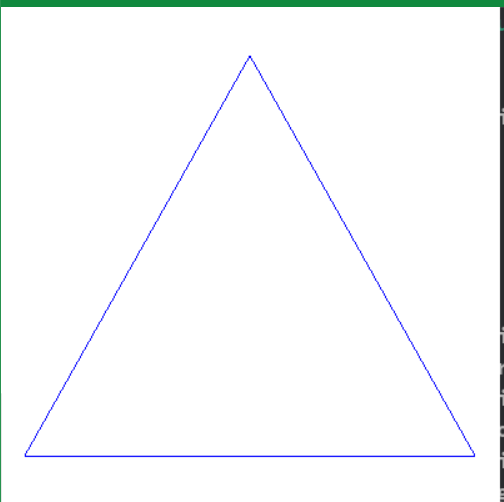
\includegraphics[width=8cm]{./2017-10-03-01.png}
\end{center}

\item 三角形の描画\\

\begin{center}

\includegraphics[width=8cm]{./2017-10-03-02.png}
\end{center}

\item 複数の図形の描画\\

\begin{center}
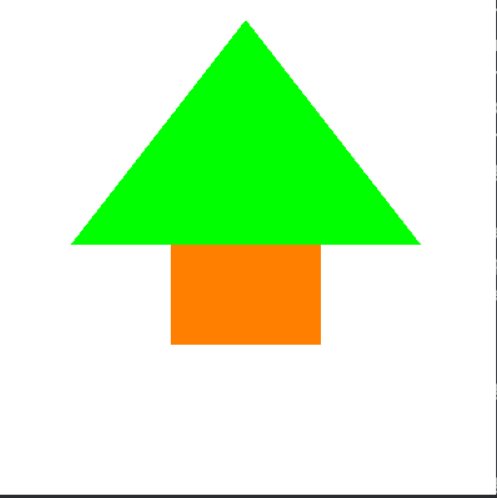
\includegraphics[width=8cm]{./2017-10-03-03.png}
\end{center}

\item ループ処理を用いた描画\\

\begin{center}
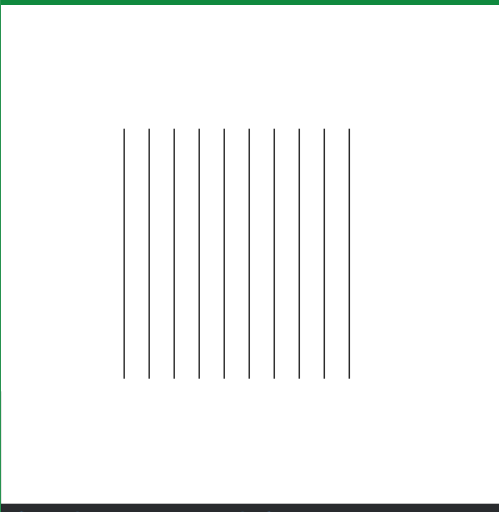
\includegraphics[width=8cm]{./2017-10-03-04.png}
\end{center}

\item 円の描画\\

\begin{center}
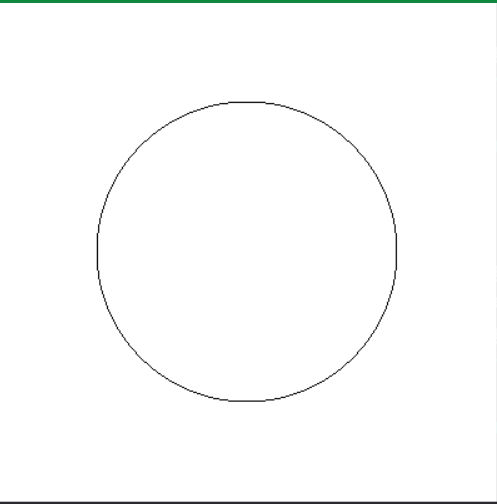
\includegraphics[width=8cm]{./2017-10-03-05.png}
\end{center}
\end{enumerate}

\subsection{サンプルコード}
\label{sec:org4008bbf}
\begin{enumerate}
\item ウインドウの表示\\

\begin{minted}[frame=lines,linenos=true,obeytabs,tabsize=4]{c++}
#include <GL/glut.h> // ライブラリ用ヘッダファイルの読み込み

// 表示部分をこの関数で記入
void display(void) {        
  glClearColor (1.0, 1.0, 1.0, 1.0);  // 消去色指定
  glClear (GL_COLOR_BUFFER_BIT );     // 画面消去

  /* ここに描画に関するプログラムコードを入れる */

  glFlush(); // 画面出力
}

// メインプログラム
int main (int argc, char *argv[]) { 
  glutInit(&argc, argv);          // ライブラリの初期化
  glutInitWindowSize(400 , 400);  // ウィンドウサイズを指定
  glutCreateWindow(argv[0]);      // ウィンドウを作成
  glutDisplayFunc(display);       // 表示関数を指定
  glutMainLoop();                 // イベント待ち
  return 0;
}

\end{minted}

\item 直線の描画\\

\begin{minted}[frame=lines,linenos=true,obeytabs,tabsize=4]{c++}
#include <GL/glut.h> // ライブラリ用ヘッダファイルの読み込み

// 表示部分をこの関数で記入
void display(void) {        
  glClearColor (1.0, 1.0, 1.0, 1.0);  // 消去色指定
  glClear (GL_COLOR_BUFFER_BIT );     // 画面消去

  glColor3d(0.0, 0.0, 1.0);   // 色指定(R,G,B)で0~1まで
  glBegin(GL_LINE_LOOP);      // 描画するものを指定
  glVertex2d(-0.9, -0.8); // 頂点位置の指定(1つめ)
  glVertex2d( 0.9, -0.8); // 頂点位置の指定(2つめ)
  glVertex2d( 0.0,  0.8); // 頂点位置の指定(3つめ) 
  glEnd();                               

  glFlush(); // 画面出力
}

// メインプログラム
int main (int argc, char *argv[]) { 
  glutInit(&argc, argv);          // ライブラリの初期化
  glutInitWindowSize(400 , 400);  // ウィンドウサイズを指定
  glutCreateWindow(argv[0]);      // ウィンドウを作成
  glutDisplayFunc(display);       // 表示関数を指定
  glutMainLoop();                 // イベント待ち
  return 0;
}
\end{minted}

\item 三角形の描画\\

\begin{minted}[frame=lines,linenos=true,obeytabs,tabsize=4]{c++}
#include <GL/glut.h> // ライブラリ用ヘッダファイルの読み込み

// 表示部分をこの関数で記入
void display(void) {        
  glClearColor (1.0, 1.0, 1.0, 1.0);  // 消去色指定
  glClear (GL_COLOR_BUFFER_BIT );     // 画面消去

  glColor3d(0.0, 1.0, 1.0);   // 色指定(R,G,B)で0~1まで
  glBegin(GL_TRIANGLES);      // 描画するものを指定
  glVertex2d(-0.9, -0.8); // 頂点位置の指定(1つめ)
  glVertex2d( 0.9, -0.8); // 頂点位置の指定(2つめ)
  glVertex2d( 0.0,  0.8); // 頂点位置の指定(3つめ) 
  glEnd();                               

  glFlush(); // 画面出力
}

// メインプログラム
int main (int argc, char *argv[]) { 
  glutInit(&argc, argv);          // ライブラリの初期化
  glutInitWindowSize(400 , 400);  // ウィンドウサイズを指定
  glutCreateWindow(argv[0]);      // ウィンドウを作成
  glutDisplayFunc(display);       // 表示関数を指定
  glutMainLoop();                 // イベント待ち
  return 0;
}
\end{minted}

\item 複数の図形の描画\\

\begin{minted}[frame=lines,linenos=true,obeytabs,tabsize=4]{c++}
#include <GL/glut.h> // ライブラリ用ヘッダファイルの読み込み

// 表示部分をこの関数で記入
void display(void) {        
  glClearColor (1.0, 1.0, 1.0, 1.0);  // 消去色指定
  glClear (GL_COLOR_BUFFER_BIT );     // 画面消去

  // 1つ目の図形
  glColor3d(1.0, 0.5, 0.0);   // 色指定(R,G,B)で0~1まで
  glBegin(GL_QUADS);     // 描画するものを指定
        glVertex2d(-0.3,  0.0); // 頂点位置の指定(1つめ)
        glVertex2d(-0.3, -0.4); // 頂点位置の指定(2つめ)
        glVertex2d( 0.3, -0.4); // 頂点位置の指定(3つめ) 
        glVertex2d( 0.3,  0.0); // 頂点位置の指定(4つめ) 
  glEnd();                               

  // 2つ目の図形
  glColor3d(0.0, 1.0, 0.0);   // 色指定(R,G,B)で0~1まで
  glBegin(GL_TRIANGLES);      // 描画するものを指定
        glVertex2d( 0.0, 0.9); // 頂点位置の指定(1つめ)
        glVertex2d(-0.7, 0.0); // 頂点位置の指定(2つめ)
        glVertex2d( 0.7, 0.0); // 頂点位置の指定(3つめ) 
  glEnd();                               

  glFlush(); // 画面出力
}

// メインプログラム
int main (int argc, char *argv[]) { 
  glutInit(&argc, argv);          // ライブラリの初期化
  glutInitWindowSize(400 , 400);  // ウィンドウサイズを指定
  glutCreateWindow(argv[0]);      // ウィンドウを作成
  glutDisplayFunc(display);       // 表示関数を指定
  glutMainLoop();                 // イベント待ち
  return 0;
}
\end{minted}

\item ループ処理を用いた描画\\

\begin{minted}[frame=lines,linenos=true,obeytabs,tabsize=4]{c++}
#include <GL/glut.h> // ライブラリ用ヘッダファイルの読み込み

// 表示部分をこの関数で記入
void display(void) {        
  glClearColor (1.0, 1.0, 1.0, 1.0);  // 消去色指定
  glClear (GL_COLOR_BUFFER_BIT );     // 画面消去

  glColor3d(0.0, 0.0, 0.0);   // 色指定(R,G,B)で0~1まで
  glBegin(GL_LINES);
  for(int i = 0; i < 10; i++) {
    glVertex2d(i * 0.1 - 0.5,  0.5); 
    glVertex2d(i * 0.1 - 0.5, -0.5); 
  }
  glEnd();                               

  glFlush(); // 画面出力
}

// メインプログラム
int main (int argc, char *argv[]) { 
  glutInit(&argc, argv);          // ライブラリの初期化
  glutInitWindowSize(400 , 400);  // ウィンドウサイズを指定
  glutCreateWindow(argv[0]);      // ウィンドウを作成
  glutDisplayFunc(display);       // 表示関数を指定
  glutMainLoop();                 // イベント待ち
  return 0;
}
\end{minted}

\item 円の描画\\

\begin{minted}[frame=lines,linenos=true,obeytabs,tabsize=4]{c++}
#include <GL/glut.h> // ライブラリ用ヘッダファイルの読み込み
#include <math.h>

// 表示部分をこの関数で記入
void display(void) {        
  glClearColor (1.0, 1.0, 1.0, 1.0);  // 消去色指定
  glClear (GL_COLOR_BUFFER_BIT );     // 画面消去

  glColor3d(0.0, 0.0, 0.0);   // 色指定(R,G,B)で0~1まで
  glBegin(GL_LINE_LOOP);
  for(int i = 0; i < 360; i++) {
    double x = cos(i * 3.14159 /180.0);
    double y = sin(i * 3.14159 /180.0);
    glVertex2d(x * 0.6, y * 0.6); 
  }
  glEnd();                               

  glFlush(); // 画面出力
}

// メインプログラム
int main (int argc, char *argv[]) { 
  glutInit(&argc, argv);          // ライブラリの初期化
  glutInitWindowSize(400 , 400);  // ウィンドウサイズを指定
  glutCreateWindow(argv[0]);      // ウィンドウを作成
  glutDisplayFunc(display);       // 表示関数を指定
  glutMainLoop();                 // イベント待ち
  return 0;
}
\end{minted}
\end{enumerate}

\newpage

\section{課題2}
\label{sec:org3c8a7d3}
下図のように、画面内に縦に5つ、横に5つ、合計25個の三角形を表示するプログラムを作成しなさい。三角形の大きさ、色、配置の間隔は自由に決めてよい。\\


\begin{center}
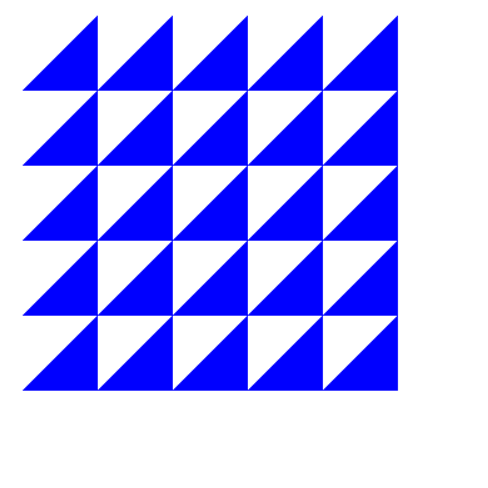
\includegraphics[width=8cm]{./2017-10-04.png}
\end{center}

\subsection{コード}
\label{sec:orgb8b8e7d}
コードから分かるように、三角形を5つ横に並べたものを次に縦に5行並べていくことで課題を解決している。\\


\begin{minted}[frame=lines,linenos=true,obeytabs,tabsize=4]{c++}
#include <GL/glut.h> // ライブラリ用ヘッダファイルの読み込み

// 表示部分をこの関数で記入
void display(void) {        
  float x = -0.6;
  float y = 0.6;
  int xcount = 0;
  int ycount = 0;

  glClearColor (1.0, 1.0, 1.0, 1.0);  // 消去色指定
  glClear (GL_COLOR_BUFFER_BIT );     // 画面消去

// 三角形5つの列を5行出力していく
  while(ycount < 5) { // 行を出力
    while (xcount < 5) { // 列を出力
      glColor3d(0.0, 0.0, 1.0);
      glBegin(GL_TRIANGLES);
      glVertex2d( x, y + 0.3); // 頂点位置の指定(1つめ)
      glVertex2d( x - 0.3, y); // 頂点位置の指定(2つめ)
      glVertex2d( x, y); // 頂点位置の指定(3つめ)
      glEnd();
      x += 0.3;
      xcount++;
    }
    xcount = 0;
    ycount++;
    x = -0.6;
    y -= 0.3;
  }
  glFlush(); // 画面出力
}

// メインプログラム
int main (int argc, char *argv[]) { 
  glutInit(&argc, argv);          // ライブラリの初期化
  glutInitWindowSize(400 , 400);  // ウィンドウサイズを指定
  glutCreateWindow(argv[0]);      // ウィンドウを作成
  glutDisplayFunc(display);       // 表示関数を指定
  glutMainLoop();                 // イベント待ち
  return 0;
}
\end{minted}

\newpage

\section{課題3}
\label{sec:orgd1320ba}
オリジナルの2次元図形を画面に表示するプログラムを作成しなさい。ただし、プログラムの中では必ず一度はforループを用いること。\\
二種類作成したため、それぞれを紹介する。\\

\subsection{円とその塗りつぶしを用いた簡単な絵の描画}
\label{sec:org27cae10}
頭と胴と目と口を描画している。\\

\begin{center}
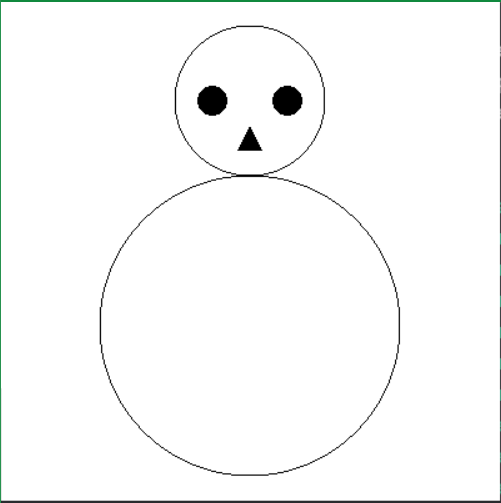
\includegraphics[width=8cm]{./2017-10-03-08.png}
\end{center}


\subsubsection{コード}
\label{sec:org749c0da}

\begin{minted}[frame=lines,linenos=true,obeytabs,tabsize=4]{c++}
#include <GL/glut.h> // ライブラリ用ヘッダファイルの読み込み
#include <math.h>

// 表示部分をこの関数で記入
void display(void) {        
  glClearColor (1.0, 1.0, 1.0, 1.0);  // 消去色指定
  glClear (GL_COLOR_BUFFER_BIT );     // 画面消去

  // 胴の描画
  glColor3d(0.0, 0.0, 0.0);
  glBegin(GL_LINE_LOOP);
  for(int i = 0; i < 360; i++) {
    double x = cos(i * 3.14159 /180.0);
    double y = sin(i * 3.14159 /180.0) - 0.5;
    glVertex2d(x * 0.6, y * 0.6); 
  }
  glEnd();

  // 頭の描画
  glColor3d(0.0, 0.0, 0.0); 
  glBegin(GL_LINE_LOOP);
  for(int i = 0; i < 360; i++) {
    double x = cos(i * 3.14159 /180.0) * 0.5;
    double y = (sin(i * 3.14159 /180.0) + 2.0) * 0.5;
    glVertex2d(x * 0.6, y * 0.6); 
  }
  glEnd();

  // 目の描画
  glColor3d(0.0, 0.0, 0.0); 
  glBegin(GL_POLYGON);
  for(int i = 0; i < 360; i++) {
    double x = cos(i * 3.14159 /180.0) * 0.1 + 0.25;
    double y = sin(i * 3.14159 /180.0) * 0.1 + 1.0;
    glVertex2d(x * 0.6, y * 0.6); 
  }
  glEnd();

  // 目の描画
  glColor3d(0.0, 0.0, 0.0); 
  glBegin(GL_POLYGON);
  for(int i = 0; i < 360; i++) {
    double x = cos(i * 3.14159 /180.0) * 0.1 - 0.25;
    double y = sin(i * 3.14159 /180.0) * 0.1 + 1.0;
    glVertex2d(x * 0.6, y * 0.6); 
  }
  glEnd();

  // 口の描画
  glColor3d(0.0, 0.0, 0.0); 
  glBegin(GL_POLYGON); 
  glVertex2d( 0.0, 0.5);
  glVertex2d( -0.05, 0.4);
  glVertex2d( 0.05,  0.4);
  glEnd();

  glFlush(); // 画面出力
}

// メインプログラム
int main (int argc, char *argv[]) { 
  glutInit(&argc, argv);          // ライブラリの初期化
  glutInitWindowSize(400 , 400);  // ウィンドウサイズを指定
  glutCreateWindow(argv[0]);      // ウィンドウを作成
  glutDisplayFunc(display);       // 表示関数を指定
  glutMainLoop();                 // イベント待ち
  return 0;
}
\end{minted}


\subsection{サイズの異なる正方形を重ね合わせた図の描画}
\label{sec:org6463f7d}
広い正方形から色を変えた少し小さな正方形を重ね合わせていく。\\

\begin{center}

\includegraphics[width=8cm]{./2017-10-04-01.png}
\end{center}
\subsubsection{コード}
\label{sec:org2169f02}

\begin{minted}[frame=lines,linenos=true,obeytabs,tabsize=4]{c++}
#include <GL/glut.h> // ライブラリ用ヘッダファイルの読み込み
#include <math.h>

// 表示部分をこの関数で記入
void display(void) {
  float x = 1.0;
  float y = 1.0;
  float color = 1.0;

  glClearColor (1.0, 1.0, 1.0, 1.0);  // 消去色指定
  glClear (GL_COLOR_BUFFER_BIT );     // 画面消去

  for (int i = 0; i < 10; ++i) {
    // 塗りつぶす色を交互に入れ替える
    if (i % 2 == 0) {
      glColor3d(color, color, color);
    }
    else {
      glColor3d(color * 0, color * 0, color * 0);
    }
    // 塗り潰す四角形の描画
    glBegin(GL_QUADS);
    glVertex2d(x, y);
    glVertex2d(-1 * x , y);
    glVertex2d(-1 * x , -1 * y);
    glVertex2d(x , -1 * y);
    glEnd();
    // 正方形のサイズを小さくする。
    x -= 0.1;
    y -= 0.1;
  }

  glFlush(); // 画面出力
}

// メインプログラム
int main (int argc, char *argv[]) { 
  glutInit(&argc, argv);          // ライブラリの初期化
  glutInitWindowSize(400 , 400);  // ウィンドウサイズを指定
  glutCreateWindow(argv[0]);      // ウィンドウを作成
  glutDisplayFunc(display);       // 表示関数を指定
  glutMainLoop();                 // イベント待ち
  return 0;
}
\end{minted}

\newpage

\section{発展課題}
\label{sec:orgb2caf4d}
「コッホ曲線」について調べ、ステップ3の時点の図形(右図)を描画するプログラムを作成しなさい。\\
コッホ曲線の定義をコードにして、繰り返し回数を3にして計算を行い、その結果を線でつないだ。\\

\begin{center}
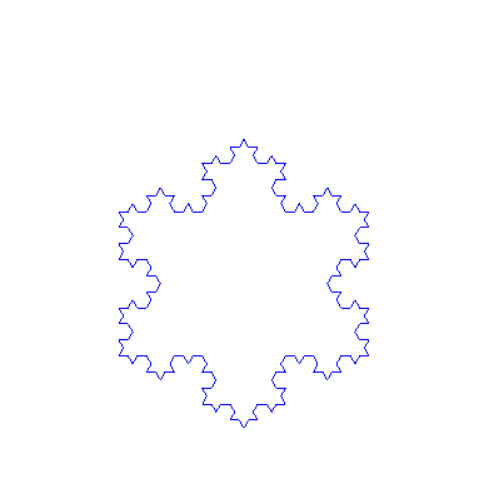
\includegraphics[width=8cm]{./2017-10-03-06.png}
\end{center}

\subsection{コード}
\label{sec:orge2d7612}

\begin{minted}[frame=lines,linenos=true,obeytabs,tabsize=4]{c++}
#include <GL/glut.h>
#include <math.h>

// 表示部分をこの関数で記入

void koch(int level, float p1x, float p1y,  float p2x, float p2y) {
  if(level == 0) {
    glColor3d(0.0, 0.0, 1.0);
    glBegin(GL_LINE_LOOP);
    glVertex2d(p1x, p1y);
    glVertex2d(p2x, p2y);
    glEnd();
    return;
  }
  float sx = (2.0 * p1x + 1.0 * p2x) / 3.0;
  float sy = (2.0 * p1y + 1.0 * p2y) / 3.0;
  float tx = (1.0 * p1x + 2.0 * p2x) / 3.0;
  float ty = (1.0 * p1y + 2.0 * p2y) / 3.0;
  float ux = (tx - sx) * (1.0 / 2.0) - (ty - sy) * (sqrt(3) / 2.0) + sx;
  float uy = (tx - sx) * (sqrt(3.0) / 2.0) + (ty - sy) * (1.0 / 2.0) + sy;

  koch(level - 1, p1x, p1y, sx, sy);
  koch(level - 1, sx, sy, ux, uy);
  koch(level - 1, ux, uy, tx, ty);
  koch(level - 1, tx, ty, p2x, p2y);
}
void display(void) {
  glClearColor(1.0, 1.0, 1.0, 1.0);
  glClear (GL_COLOR_BUFFER_BIT );     // 画面消去
  koch(3, 0.5 * 1.0, 0.5 * -1.0 * (sqrt(3.0) / 2.0),
       0.5 * -1.0, 0.5 * -1.0 * (sqrt(3.0) / 2.0));
  koch(3, -1.0 * 0.5, 0.5 * -1.0 * (sqrt(3.0) / 2.0),
       0.0 * 0.5, (sqrt(3.0) / 2.0) * 0.5);
  koch(3, 0.0 * 0.5, 0.5 * (sqrt(3.0) / 2.0),
       0.5 * 1.0, 0.5 * -1.0 * (sqrt(3.0) / 2.0));

  glFlush(); // 画面出力
}

// メインプログラム
int main (int argc, char *argv[]) { 
  glutInit(&argc, argv);          // ライブラリの初期化
  glutInitWindowSize(400 , 400);  // ウィンドウサイズを指定
  glutCreateWindow(argv[0]);      // ウィンドウを作成
  glutDisplayFunc(display);       // 表示関数を指定
  glutMainLoop();                 // イベント待ち
  return 0;
}
\end{minted}


\section{感想}
\label{sec:orgc3b07da}
特に課題に関しての感想はないが、開発環境などの構築に戸惑っている生徒が非常に多かったため、なんらかの救済策があればよいと思いました。\\
\end{document}
